\chapter{Results and Discussion}
\label{chap4:results_and_discussion}

The present chapter focuses on the experimental and practical side of this dissertation. In it, one can expect to find results for both state-of-the-art and proposed methods, as well as, the conclusions that each entails. To that end, section \ref{sec:chap4_datasets_and_working_scenario} describes the datasets used; subsections \ref{sec:chap4_method_a_results} and \ref{sec:chap4_method_b_results} assess the performance of both proposed methods; section \ref{sec:chap4_conclusion} presents some final remarks.

\section{Datasets and Working Scenario}
\label{sec:chap4_datasets_and_working_scenario}
As mentioned above, the proposed framework is composed of two modules: $\mathbf{1}$) one for recognition and $\mathbf{2}$) the other for explanation purposes. Regarding the former, the chosen \ac{CNN} is solely trained on the \ac{UBIPr} dataset \cite{ubipr}, which provides the ID annotations used in the identity verification problem. Regarding the explanation step, it mainly relies on a combination of \ac{UBIPr} and \ac{FFHQ} \cite{stylegan}. Despite not being directly applicable to the context of this work (i.e., it contains full face images, thus requiring extra steps to extract the periocular region), the \ac{FFHQ} dataset contains a large variety in terms of periocular attributes, some of which are scarcer in the \ac{UBIPr} dataset. In practice, a small, but curated, portion of the \ac{FFHQ} samples was used to create a data super set (Fig. \ref{fig:dataset_samples}). Regardless of their source, all images were resized to a common shape, depending on the task (i.e., $512$x$512$x$3$ for Mask \ac{R-CNN}, $256$x$256$x$3$ for Style\ac{GAN}$2$ and $128$x$128$x$3$ for the \ac{CNN}s).

\begin{figure}[H]
  \begin{center}
  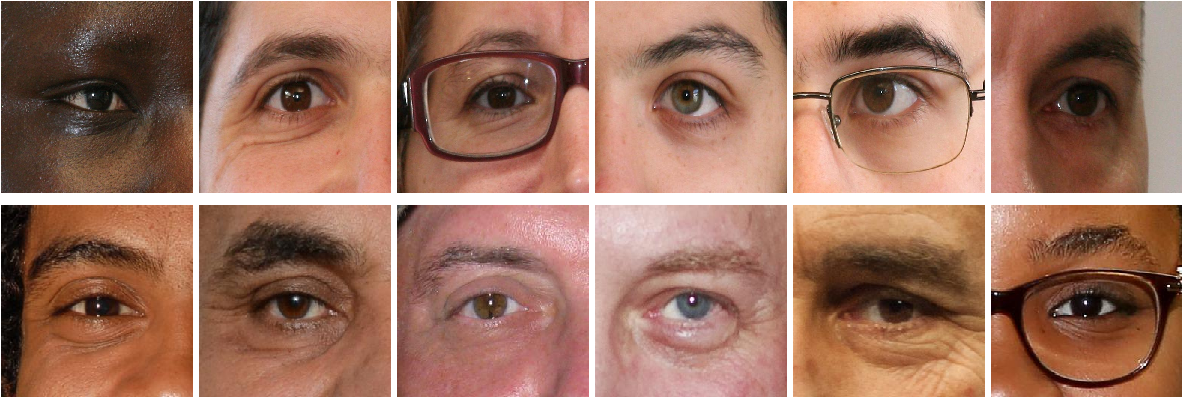
\includegraphics[width=0.70\textwidth]{figures/figure_32.pdf}
  \caption{Samples from the two datasets used. The top row represents images of the \ac{UBIPr} dataset, whereas the bottom row illustrates cropped samples of the \ac{FFHQ} dataset.}
  \label{fig:dataset_samples}
  \end{center}
\end{figure}
 As it is usual in the biometric recognition context, it is important to define proper working modes and world settings, for which the system is built. With respect to the working mode, our model runs in verification mode (also referred to as \textit{one-to-one}), where the system validates a claimed identity~\cite{introduction_to_biometric_recognition}. As for the world setting, we assume an open-world setting, in which unseen subjects can be faithfully handled in the inference step.

\section{Deep Adversarial Framework for Visually Explainable Recognition}
\label{sec:chap4_method_a_results}

\subsection{Explainability Evaluation}
\label{subsec:chap4_explainability_evaluation}

To justify the pursuit of new explainable techniques, one must start by exploring existing methods. Thus, model-specific (HL and Saliency Maps) and model-agnostic techniques (\ac{LIME} and \ac{SHAP}) were employed, so as to give a general overview of what is achievable with currently available approaches. Apart from HL (which used a ResNet-$101$ model), the techniques were paired with the same DenseNet-$121$ network. Regardless of the architecture, the task was to output the class of an image pair: "genuine" or "impostor".

The DenseNet-$121$ model was trained for $15$ epochs with a learning rate of $0.0002$ and $32$ samples per batch. Regarding the ResNet training procedure, it comprised $5$ epochs, a batch size of $32$ and a learning rate of $0.001$. Excluding Saliency Maps, the remaining techniques rely on pre-defined hyper-parameters. As such, \ac{LIME} was set to show the top $100$ super-pixels and was allowed $20000$ perturbed samples; Kernel\ac{SHAP} used $100$ segments/super-pixels and $10000$ samples; HL was trained with four discoverable parts. Finally, note that for \ac{LIME}, \ac{SHAP} and HL, the official implementations were used \footnote{https://github.com/marcotcr/lime}\footnote{https://github.com/slundberg/shap}\footnote{https://github.com/zxhuang1698/interpretability-by-parts}\\

Saliency Maps are, essentially, greyscale images where whiter tones highlight crucial areas used by the \ac{CNN} to predict a class. Accordingly, in Fig. \ref{fig:impostor_pairs_saliency_maps}, the first pair is explained by highlighting subject $B$'s glasses while, in the second pair, subject $A$'s eyebrow definitely justifies a non-match decision (just like a skin spot in subject $B$'s sample, which this technique fails to identify). Moving to the bottom row, pair number three is clearly explained by accentuating one of the irises and the fourth pair is explained through the differences in the eyebrow regions (albeit, not as detrimental as the skins could have been).

Overall, Saliency Maps provide relatively easy explanations to otherwise opaque models, and manage to outline big components (like the eyebrow or iris), while at the same time, leaving behind skin spots and equally small, but relevant, features.

\begin{figure}[H]
\centering
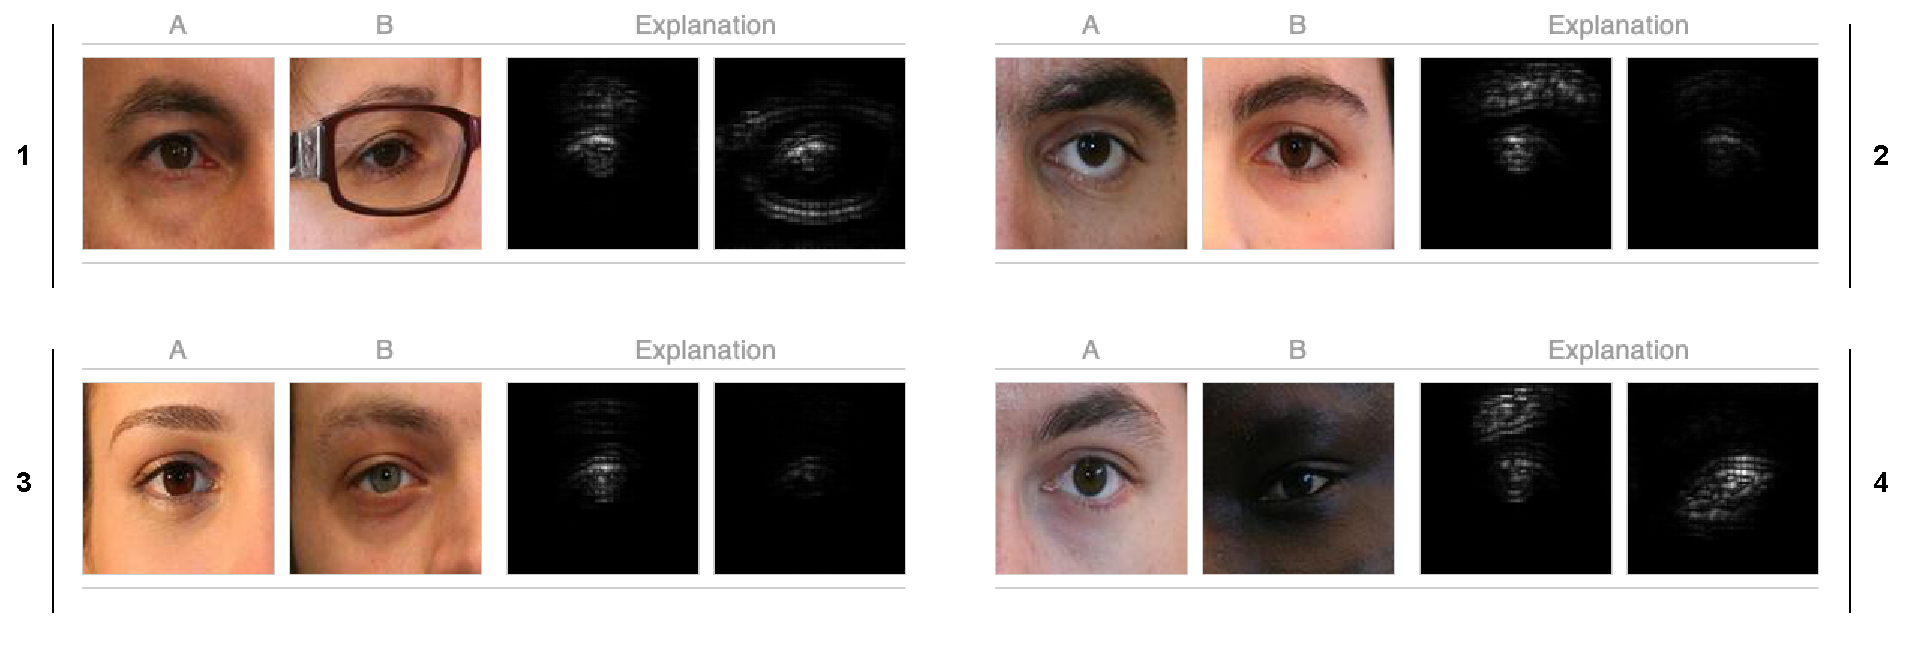
\includegraphics[width=410pt]{figures/figure_33.pdf}
\caption{Impostor pairs explained using Saliency Maps. Whiter tones highlight areas that justify the predicted class.}
\label{fig:impostor_pairs_saliency_maps}
\end{figure}

\ac{LIME}, as previously mentioned, divides images into super-pixels that are either kept or disabled. With effect, in Fig. \ref{fig:impostor_pairs_lime}, the first pair's explanation includes a portion of person $B$'s glasses and, in the second pair, a disparity in terms of eyebrows is somewhat manifested. As for pairs three and four, the former is explained by keeping super-pixels that comprise subject $A$'s eyebrow (but missing those that include the irises), while the latter's explanation preserves some skin super-pixels. 

Similarly to Saliency Maps, \ac{LIME} generates passable explanations, meaning that it highlights at least one major feature, but failing to be consistently incisive, in our experiments.

\begin{figure}[h]
\centering
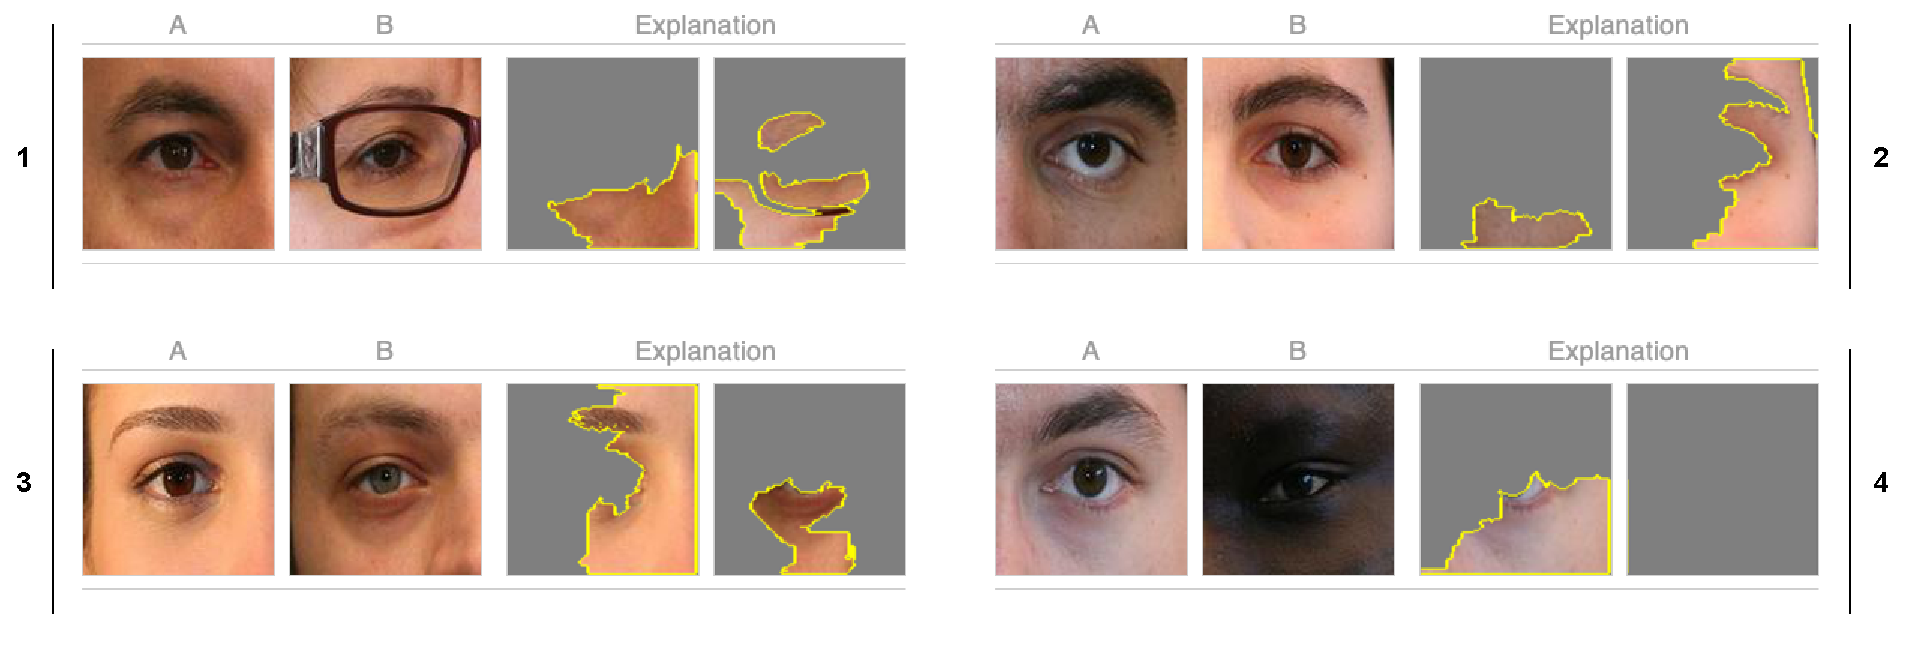
\includegraphics[width=\textwidth]{figures/figure_34.pdf}
\caption{Impostor pairs explained with \ac{LIME}. As mentioned earlier, \ac{LIME} keeps the most favourable super-pixels and replaces the remaining ones with a solid colour.}
\label{fig:impostor_pairs_lime}
\end{figure}

Kernel\ac{SHAP}, on the other hand, produces results with various shades of green and red, depending on how favourable (red) or not (green) the highlighted super-pixels are to the predicted "impostor" class. As before, the first pair is explained with the presence or absence of glasses and the second with the eyebrows and a portion of the skin. As for pair number three, both irises are shaded with a slight red tone, just like the eyebrows. Lastly, regarding the fourth pair, a major skin area, belonging to person $B$, is accurately painted in red (even though some of the skin portrays either green or very slight red tones).

In general, this implementation of \ac{SHAP} (i.e., Kernel\ac{SHAP}) is able to colour specific features in an image based on how likely they are to change the "impostor" class. Despite missing some features (e.g., some skin areas), the overall results are satisfactory, with some room for improvement.

\begin{figure}[h]
\centering
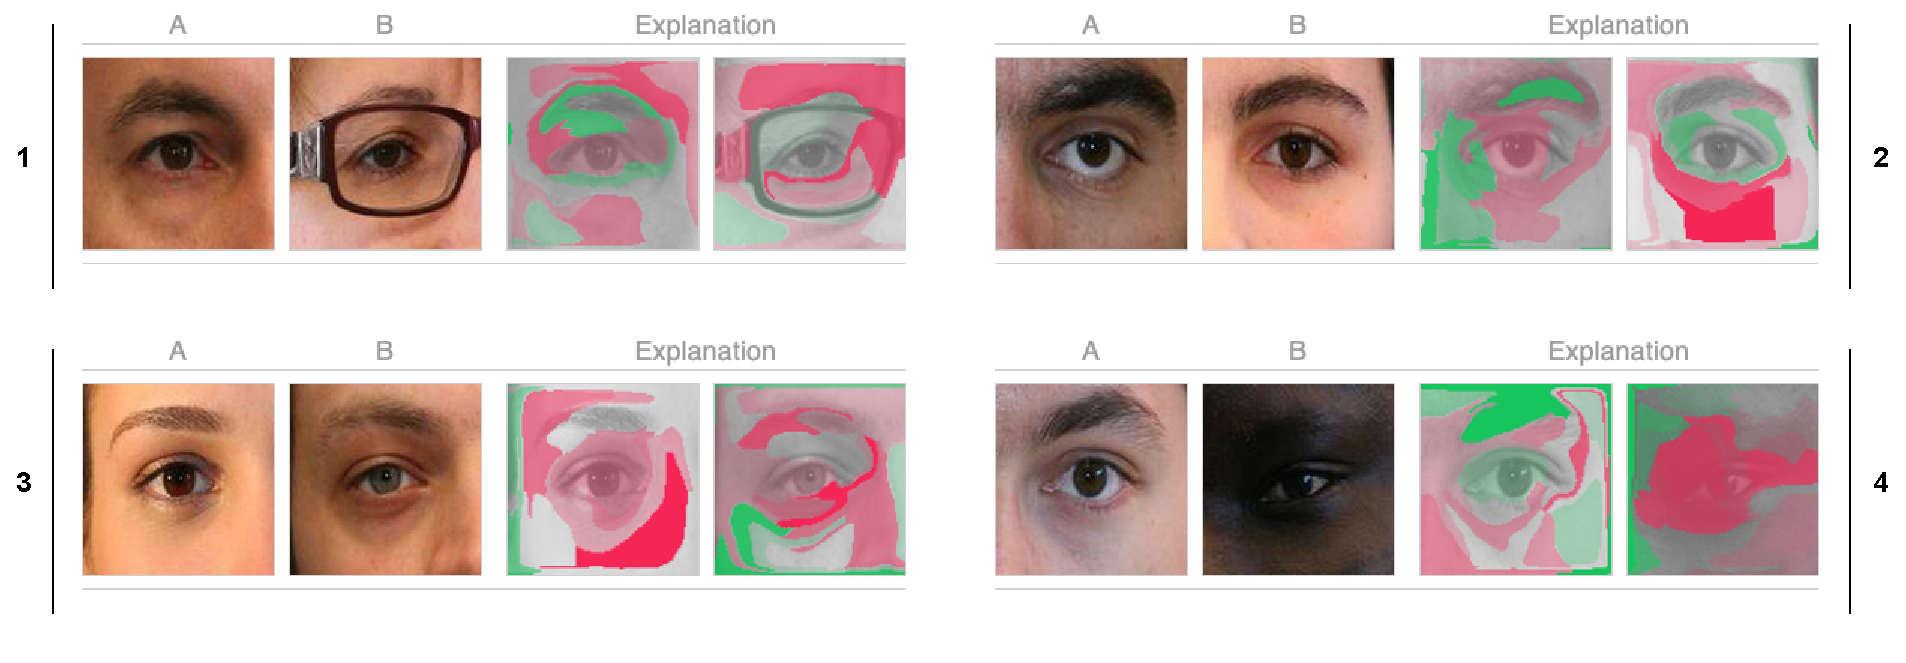
\includegraphics[width=\textwidth]{figures/figure_35.pdf}
\caption{Impostor pairs explained with \ac{SHAP}. \ac{SHAP} diverges from \ac{LIME} by highlighting certain areas with red or green tones, depending on whether they increase or decrease the probability of the output class.}
\label{fig:impostor_pairs_shap}
\end{figure}

Finally, as described in \cite{interpretability_by_parts}, HL produces intuitive heat maps as a form of explainability. In Fig. \ref{fig:impostor_pairs_by_parts}, pair one is rightly explained by colouring one of the eyebrows and the glasses with red tones. Pair number two remains accurate by strongly identifying both eyebrow as being different, in addition to the eyelashes. As pleasing as the top two results are, the third explanation unfortunately fails to capture obvious differences in iris colour, amongst other possible explanations. Pair number four concludes this method's results with an acceptable explanation, in the sense that the skins are largely ignored in favour of the eyebrows.

HL delivers readable results, mostly aided by a clear indication of which areas are regarded as important. Unfortunately, some features are not displayed in a sufficiently prominent manner (e.g., the skin in the fourth sample), leading to partial explanations.

\begin{figure}[h]
\centering
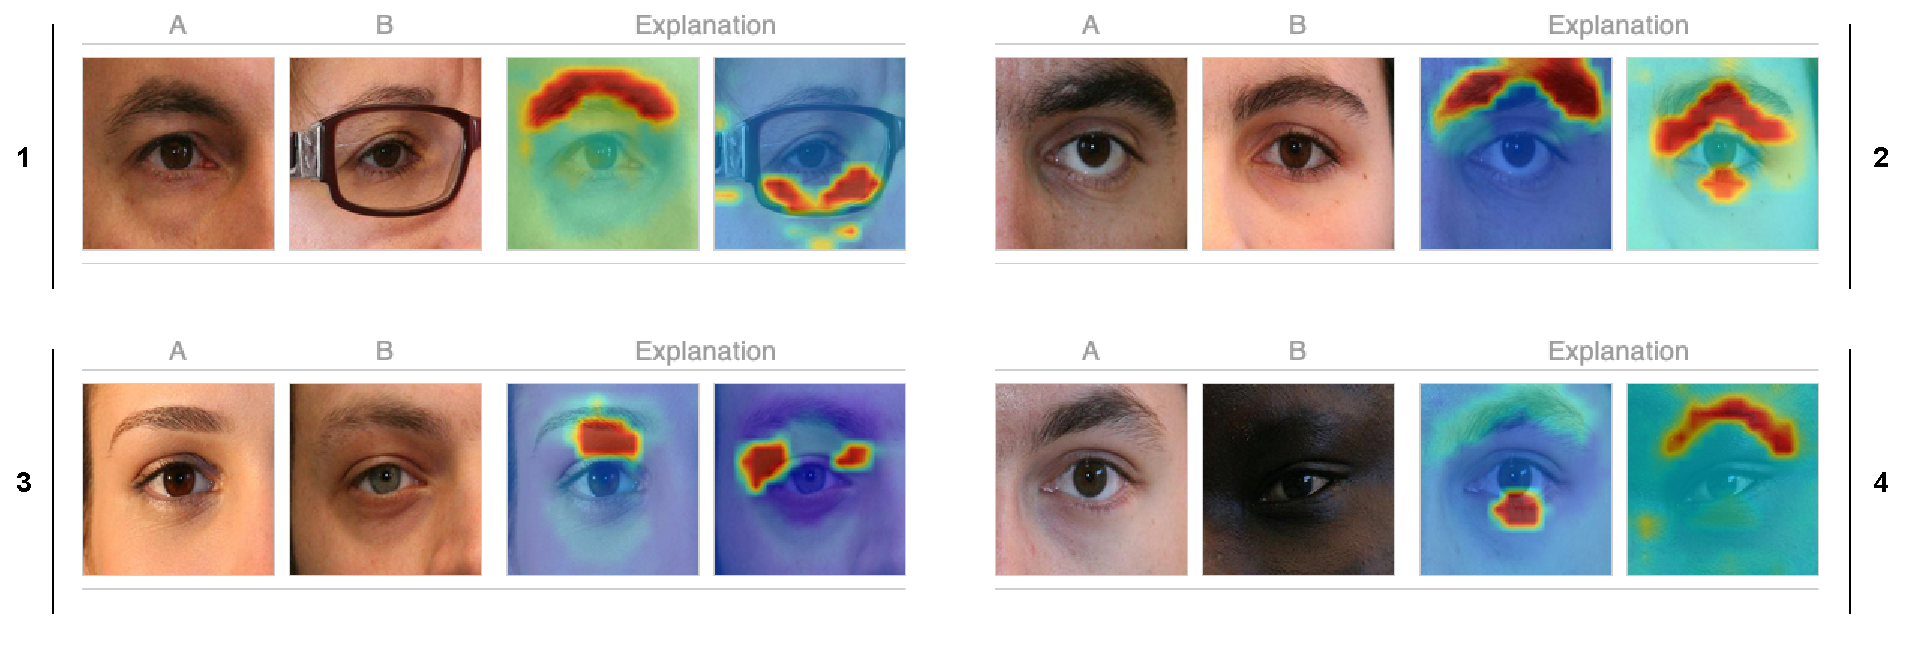
\includegraphics[width=\textwidth]{figures/figure_36.pdf}
\caption{Impostor pairs explained with the method by Huang and Li. Such method produces heat maps in which red areas are the most significant.}
\label{fig:impostor_pairs_by_parts}
\end{figure}

These results are already decent and certainly keep explainability at the forefront. However, there are cases where these techniques miss obvious components, and we argue improvements can be made with approaches that are specifically designed to address this type of problem. \\

Considering the points established above, our deep framework attempts to produce both readable and effective results. As seen in Fig. \ref{fig:method_a_results}, our explanations follow the same colour coding as Kernel\ac{SHAP} (i.e., green for irrelevant features and red for relevant ones). We produce immediately discernible explanations, highlighting, where applicable, eyebrows, irises, skins, glasses and skin spots. More specifically, to explain the first pair our approach gave emphasis to the glasses and, to a lesser scale, person $A$'s skin texture. For pair number four, the explanation shows how decisive the skins were to an "impostor" decision, while in pair five one of the eyelids and both eyebrows are shown to be different. Furthermore, an obvious disparity in eyebrow thicknesses is clearly portrayed in pair six, while pair eight is perhaps the pinnacle of what our method can highlight: contrasting iris colours and the totally different eyebrows. Finally, the last row contains samples with generally accurate explanations, thus proving our solution's effectiveness.

In broad terms, we argue that our approach delivers explanations that are easy to understand, categorically stating \emph{why} a decision was taken (in this case, "impostor"). 

\begin{figure}[H]
\centering
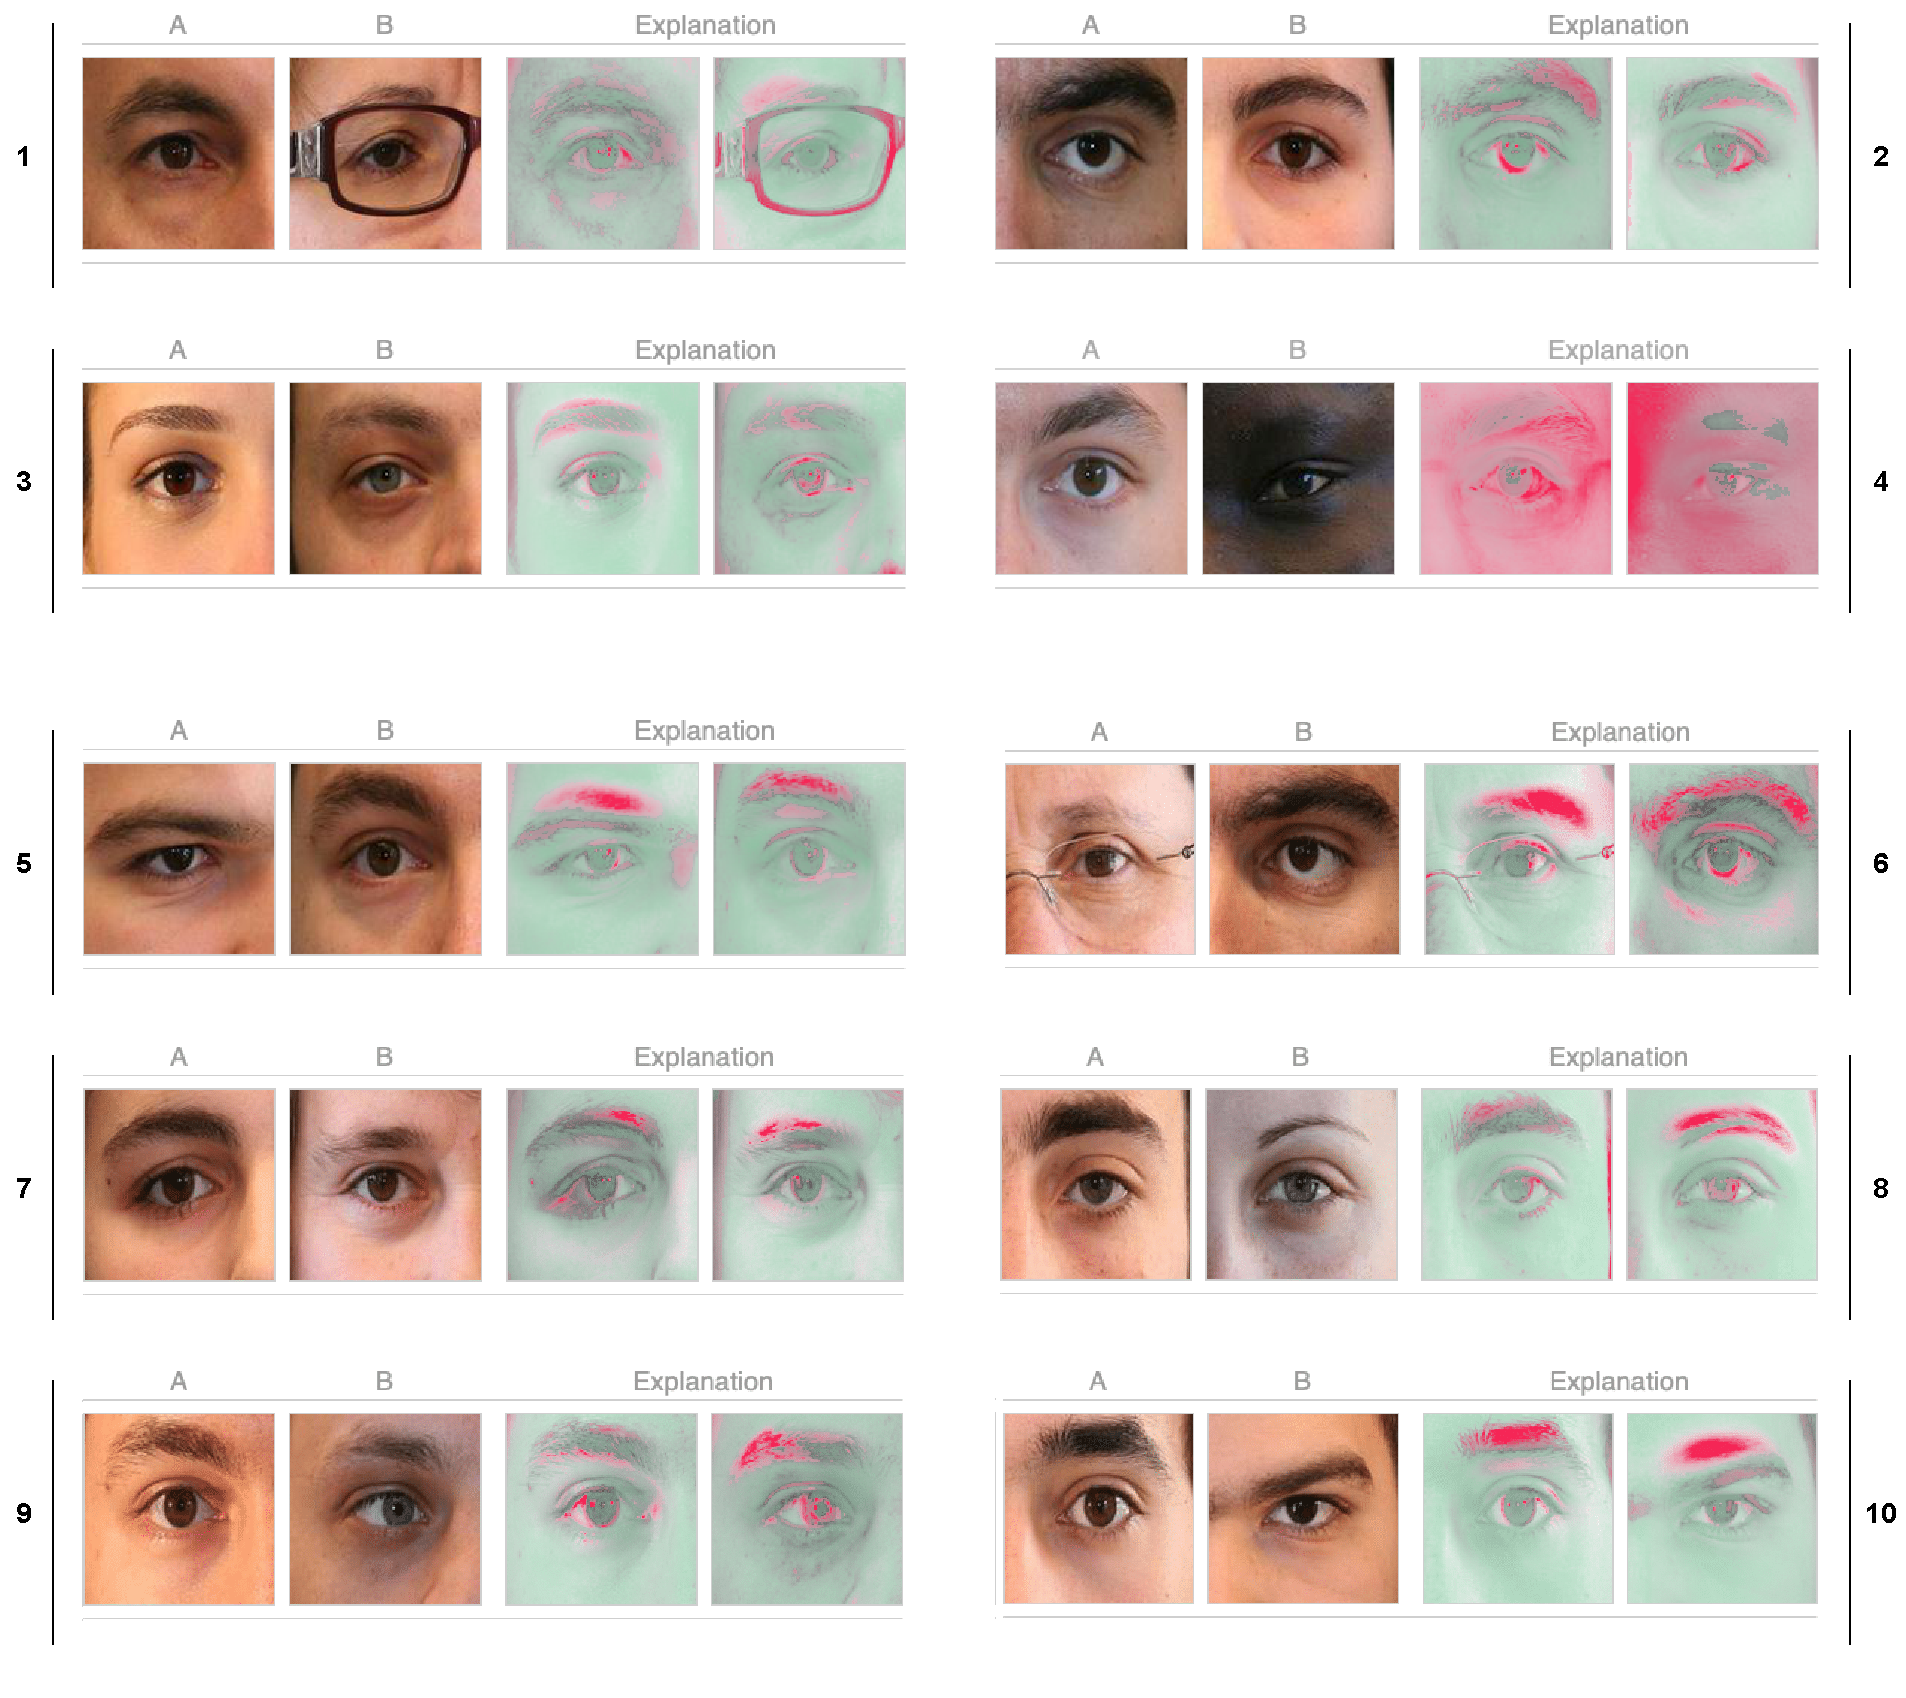
\includegraphics[width=\textwidth]{figures/new_figure_37.pdf}
\caption{Results obtained with the first method. The top four pairs can be directly compared with the results seen in Figs. \ref{fig:impostor_pairs_saliency_maps}, \ref{fig:impostor_pairs_lime}, \ref{fig:impostor_pairs_shap} and \ref{fig:impostor_pairs_by_parts}, whereas the bottom six pairs are exclusive to our method, so as to test it against a broader set.}
\label{fig:method_a_results}
\end{figure}

When objectively measuring the differences between the explanations provided by the proposed method and the baselines (\ac{LIME}, \ac{SHAP}, Huang and Li (HL) and  Saliency Maps (SM)), we used a set of $100$ heterogeneous test queries and measured the pixel-wise explanation coefficients returned by each technique, which correspond to the importance (weight) given by each method to a particular image position for a decision. Next, considering that any meaningful correlations between the responses of two methods would have to be linear, we measured the Pearson's linear correlation between pairs of techniques:
\begin{equation}
    r_{xy} = \frac{\sum_i (x_i - \hat{x}) (y_i -\hat{y})}{\sqrt{\sum_i (x_i -\hat{x})^2 \sum_i (y_i -\hat{y})^2}},
\label{eq:neighbour_score}
\end{equation}
where $x_i/y_i$ denote the i$^{th}$ scores provided by each technique and the $\hat{.}$ symbol denotes the mean value. This way, $r_{xy}$ measures how similar are the explanations provided by the $x$ and $y$ techniques: values close to $0$ will correspond to more independent explanations, while values towards $1$ will point for semantic similarities between the explanations provided by both techniques.\\

\begin{figure}[h]
  \begin{center}
  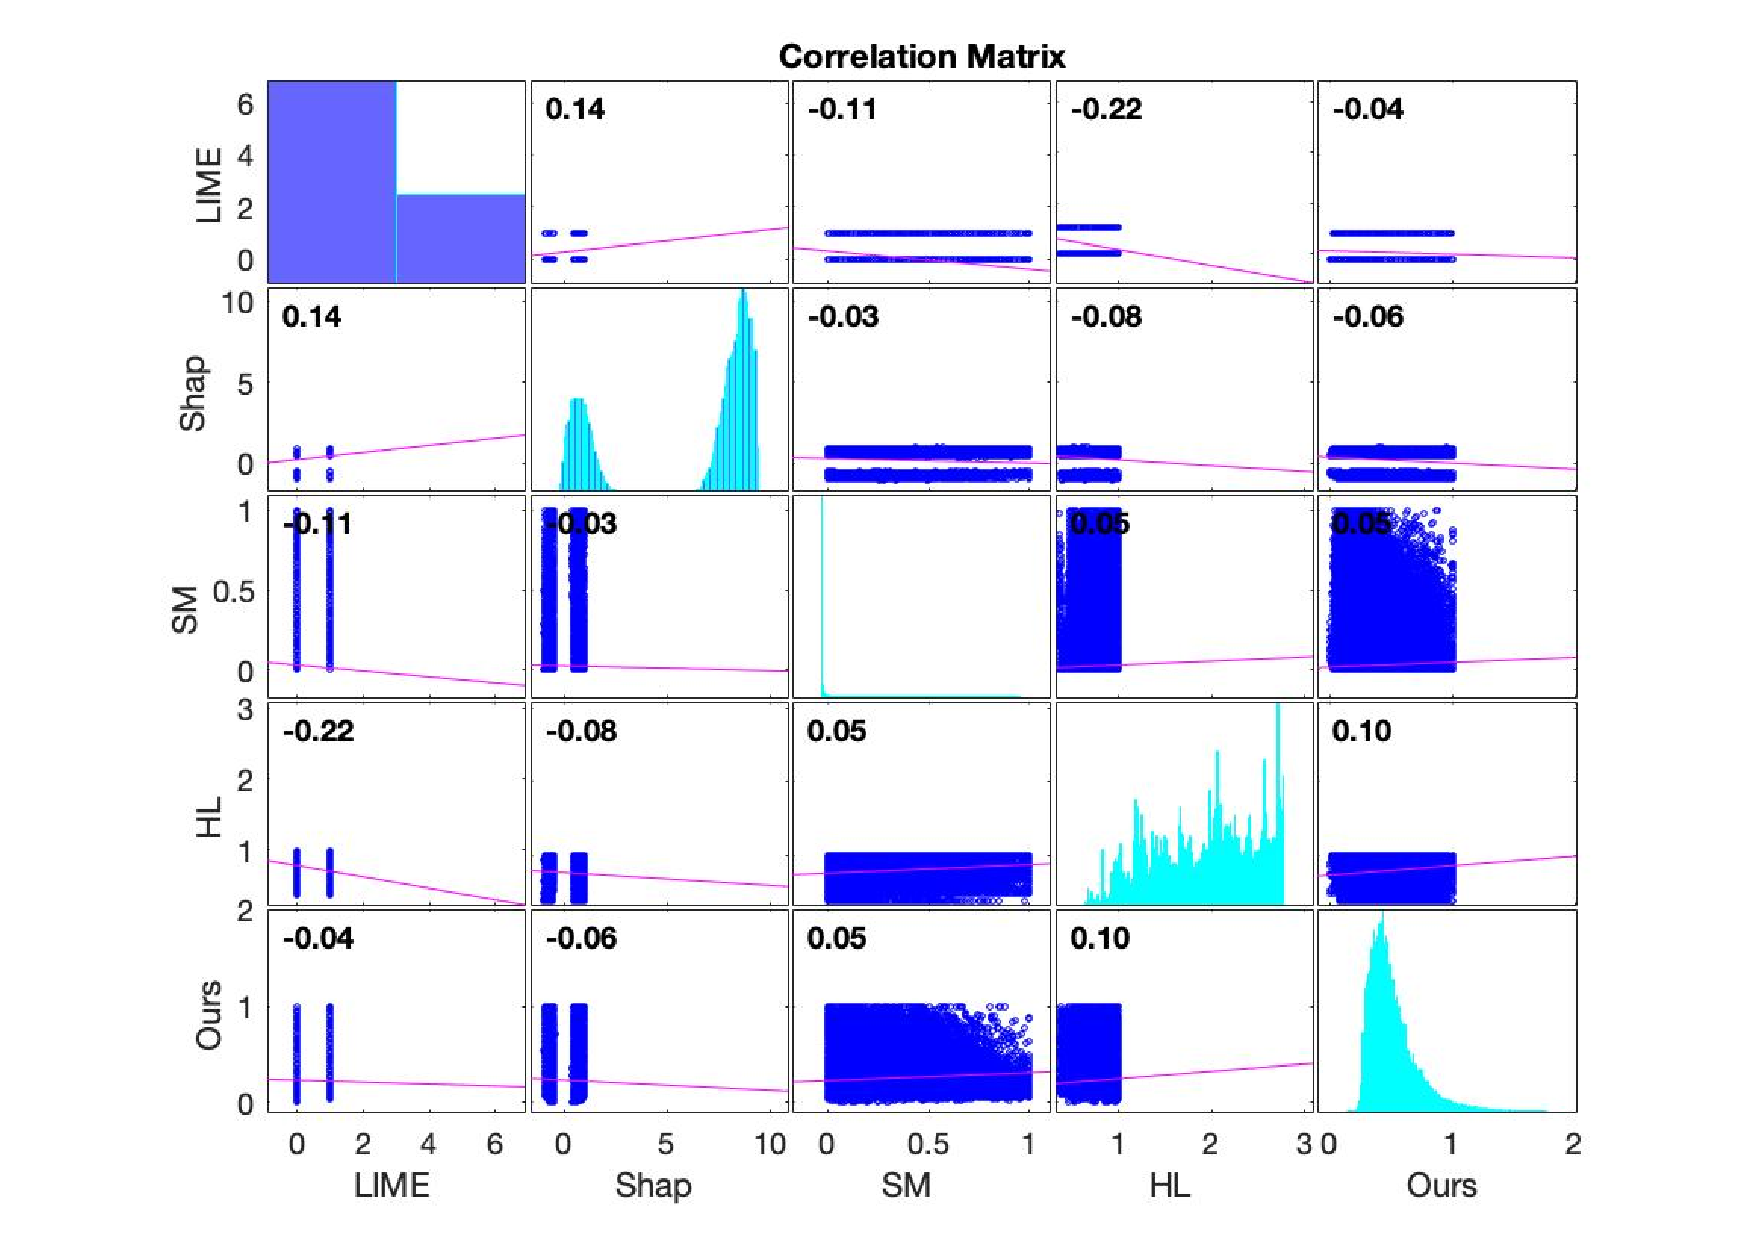
\includegraphics[width=0.9\textwidth]{figures/figure_38.pdf}
  \caption{Pearson  correlation  values  between  the  pixel-wise  responses provided by the method proposed in this document (Ours) and four baselines techniques (\ac{LIME}, \ac{SHAP}, Huang and Li (HL) and Saliency Maps (SM)).}
  \label{fig:confusion_matrices}
  \end{center}
\end{figure}

The results are conveyed through the confusion matrices shown in Fig. \ref{fig:confusion_matrices}, where the main diagonal provides the distributions of the scores generated by each technique and the remaining cells provide the scatter plots between pairs of techniques with the Pearson's correlation value $r_{xy}$ given at the top-left corner of each cell ("SM" stands for Saliency Maps and "HL" denotes the Huang and Li solution)). All these techniques report a local numeric value that corresponds to the role/importance of each region in the final decision. The exception is \ac{LIME}, where the pixels are discriminated in a binary manner (i.e., "visible" or "occluded"). In this case, we consider "visible" to be equal to $1$ and "occluded" to $0$.

Overall, we observed that the techniques provide relatively independent responses for the importance given to each pixel in the final decision. Interestingly, in some cases, there are even negative correlation values between two methods (e.g., HL and \ac{LIME} or SM and \ac{LIME}). There are other pairs of solutions that achieved almost full independence between their responses (the Shapley/Ours methods), which points for completely different strategies being used to define the explaining regions/features. Regarding our method, its levels of correlation were kept relatively low with respect to the remaining methodologies, achieving values of  $0.24$ with respect to the method of Huang and Li (the most correlated), and $0.1$ for Saliency maps. Still, we conclude that the proposed solution is extracting  semantic information (e.g., features and regions) of the vicinity of the human eye that is evidently different of the kind of information emphasised  by any of the remaining methods, which supports the usefulness of the solution described in this document.

\subsection{Recognition Accuracy Evaluation}
\label{subsec:chap4_recognition_accuracy_evaluation}

At first, note that we do not aim at providing a better recognition framework than the state-of-the-art, in terms of the recognition rates.  Even though, our main purpose in this section was to perceive if the proposed recognition/explanation network is able to achieve competitive recognition performance with respect to the state-of-the-art.\\

We compare the recognition effectiveness of the proposed method with respect to a well known periocular recognition model (due to Zhao and Kumar~\cite{accurate_periocular_recognition},  considered to represent the state-of-the-art). In order to assess the performance of both methods, the \ac{EER} and \ac{AUC} metrics were used.

On one hand, \ac{EER} measures the threshold at which we have an equality between a system's \textit{false acceptance rate} (i.e., the percentage of samples in which the system output a $1$ when it should have been a $0$) and \textit{false rejection rate} (i.e., the percentage of samples that a system classifies as $0$ when they are, in fact, of class $1$). Ideally, the \ac{EER} should be as small as possible, therefore indicating that a system is highly accurate.

On the other hand, \ac{AUC} is typically applied on binary systems (like ours) and it quantifies the system's ability to distinguish between classes. To compute such metric, we must start by obtaining a \ac{ROC} curve (similar to the one shown in Fig. \ref{fig:roc_curve}). This graph plots the relation between \ac{TPR} and \ac{FPR} values at many different decision thresholds (i.e, the values beneath which our systems considers a sample to be of class $0$ and above which the sample belongs to class $1$). \ac{AUC}, as the name suggests, stands for the area directly beneath the \ac{ROC} curve. In a perfect situation, the curve would touch the  ($0$, $1$) point and the area would obviously be $1$. Conversely, a random classifier would be closer to the red dashed line in Fig. \ref{fig:roc_curve}, meaning that no threshold would save it from being a bad model.\\

Using the UBIRIs.v$2$ set \cite{ubiris_v2} and the learning/evaluation protocols described in \cite{accurate_periocular_recognition}, we obtained the results summarised in Table \ref{tab:quantitative_evaluation}. Also, we provide \ac{ROC} values of the proposed strategy, that can be fairly combined with the similar \ac{ROC} plot provided by the original authors of the baseline in~\cite{zhao_kumar_novel}.

A bootstrapping-like strategy was used, by sampling $90$\% of the available data in UBIRIS.v$2$ and dividing the resulting samples between two disjoint sets: $80$\% for training and the remaining $20$\% for test. The models were trained separately in each sample and the performance evaluated in the corresponding test set, from where the \ac{EER} and \ac{AUC} scores were obtained. This process was repeated $10$ times, to perceive the mean $\pm$ standard deviation values for both metrics. Overall, results were satisfactory, particularly considering that - due to our modular design - the recognition module of the proposed framework can be easily replaced by any other, while keeping its explainability abilities.\\

\begin{table}[!h]
\small
{\renewcommand{\arraystretch}{1.5}%
\begin{center}
 \begin{tabular}{|c | c | c|} 
 \hline
 \textbf{Method} & \textbf{\ac{EER}} & \textbf{\ac{AUC}} \\
 \hline
 \hline
 Ours (open-world) & $0.108 \pm 3\mathrm{e}{-2}$ & $0.813 \pm 5\mathrm{e}{-2}$ \\
 Ours (closed-world) & $\mathbf{0.087 \pm 2\mathrm{e}{-2}}$ & $\mathbf{0.910 \pm 2\mathrm{e}{-2}}$ \\
 Zhao and Kumar \cite{accurate_periocular_recognition} & $0.109 \pm 2\mathrm{e}{-3}$ & $-$ \\[1.5pt]
 \hline
\end{tabular}
\end{center}}
\caption{Comparison between the recognition rates attained by the proposed method (in both world settings) and a state-of-the-art method (strictly operating in an open-world setting). Results are given for the same learning/test sets of the UBIRIS.v$2$ dataset.}
\label{tab:quantitative_evaluation}
\end{table}

For reference purposes, Fig. \ref{fig:roc_curve} provides the \ac{ROC} curve of our solution. When drawing comparisons with the corresponding results reported by authors in~\cite{accurate_periocular_recognition} in the same set, it can be seen a close recognition summary performance between both methods (summarised in Table~\ref{tab:quantitative_evaluation}). Overall, we observed a similar performance between these techniques in this dataset, which supports the idea that the proposed solution is able to approach state-of-the-art recognition rates.

\begin{figure}[h]
  \begin{center}
  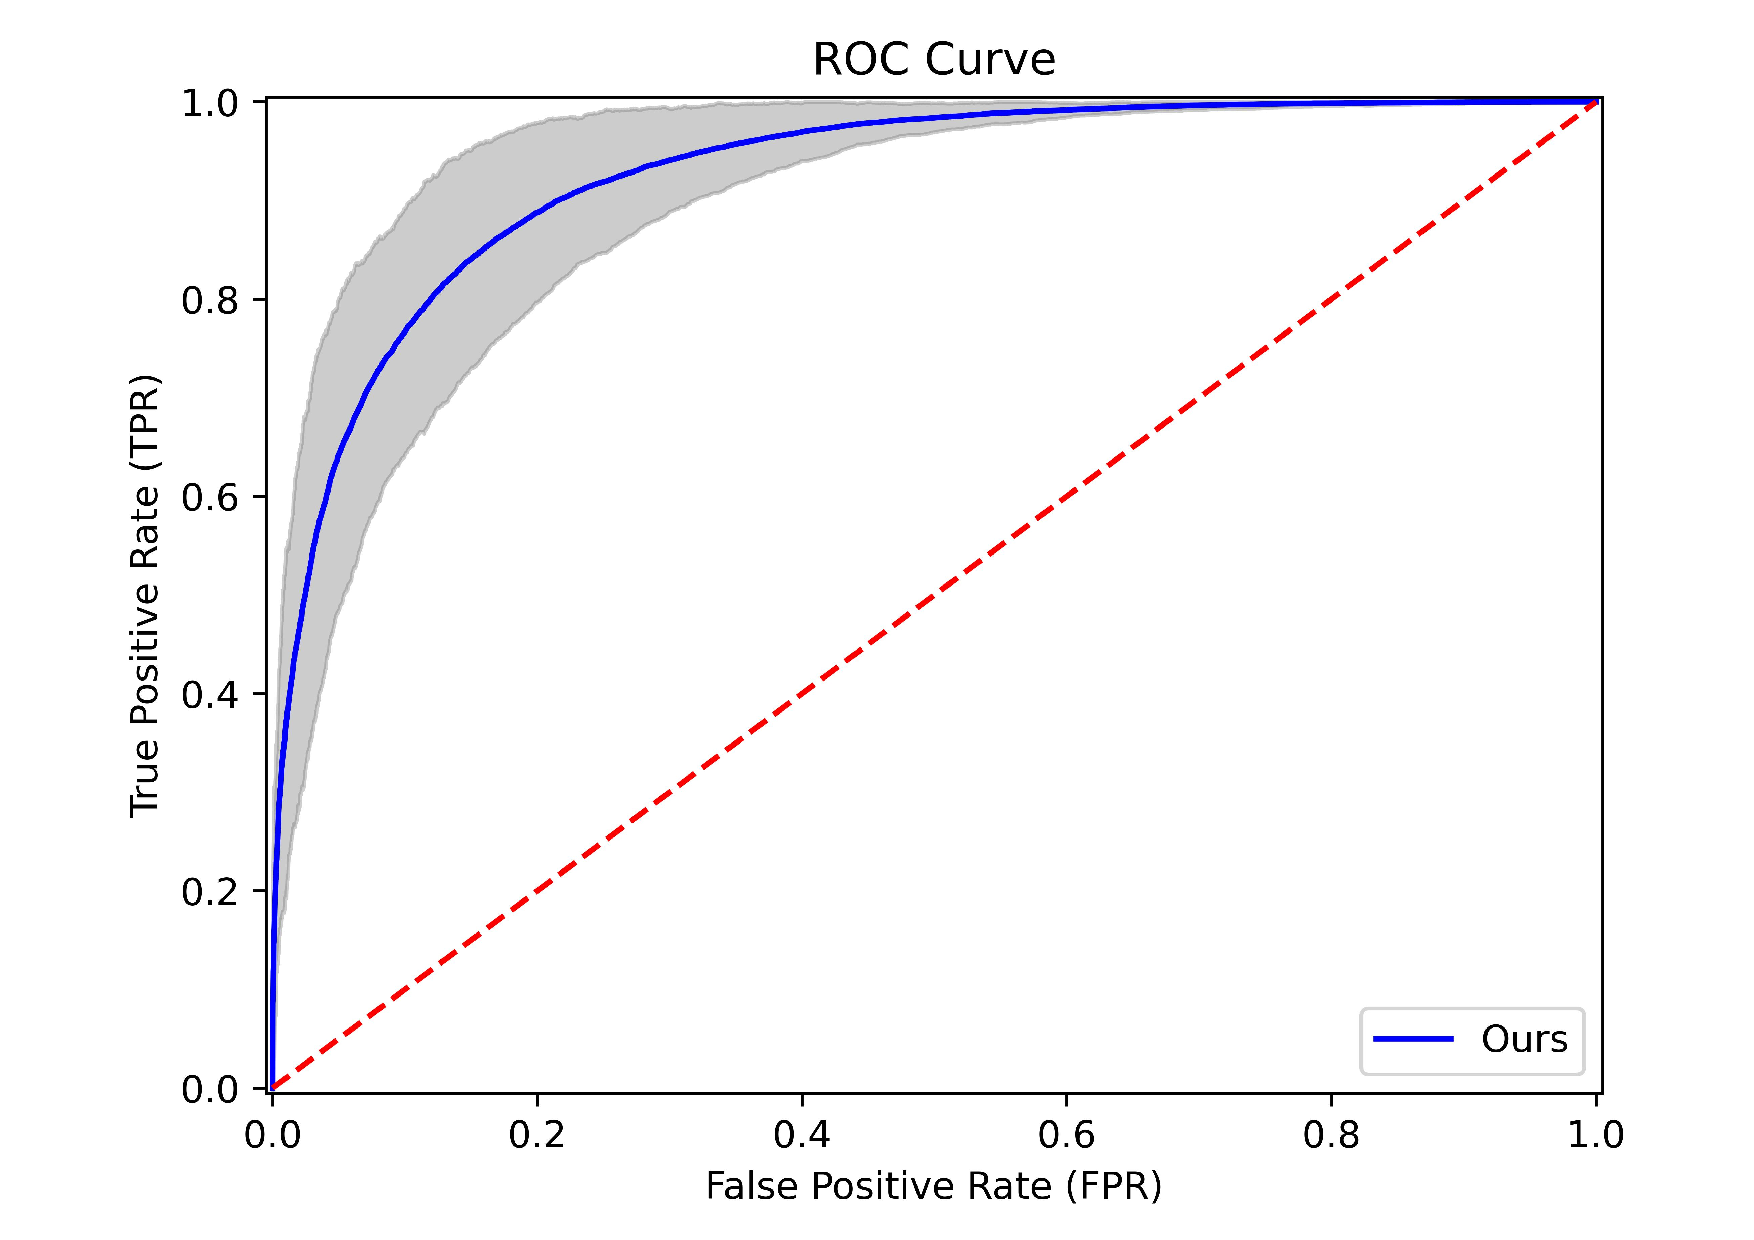
\includegraphics[width=0.7\textwidth]{figures/figure_39.pdf}
  \caption{\ac{ROC} curve obtained for the proposed method in data of the UBIRIS.v$2$ set, according to the empirical protocol designed by Zhao and Kumar \cite{accurate_periocular_recognition}. The \ac{ROC} curve corresponds to \ac{EER} and \ac{AUC} values of about $0.108$ and $0.813$, respectively.}
  \label{fig:roc_curve}
  \end{center}
\end{figure}

\subsection{Inference Time Evaluation}
\label{subsec:chap4_inference_time_evaluation}

Besides explainability and accuracy metrics, one can assess the time span that any given technique needs to produce an explanation. As such, Table \ref{tab:inference_times_evaluation} presents the inference times attained by each method in $10$ randomly sampled test pairs (so as to obtain mean $\pm$ standard deviation values):

\begin{table}[!h]
\small
{\renewcommand{\arraystretch}{1.5}%
\begin{center}
 \begin{tabular}{|c | c | c|} 
 \hline
 \textbf{Method} & \textbf{Inference Time (m)}\\
 \hline
 \hline
 Saliency Maps (SM) \cite{saliency_maps} & $15.71 \pm 0.24$ \\
 \ac{LIME} \cite{lime} & $3.64 \pm 0.05$ \\
 \ac{SHAP} \cite{shap} & $3.14 \pm 0.04$ \\
 Huang and LI (HL) \cite{interpretability_by_parts} & $\mathbf{0.08 \pm 0.01}$ \\
 Ours & $3.23 \pm 1.75$ \\
 \hline
\end{tabular}
\end{center}}
\caption{Comparison between the mean inference times (in minutes) attained by our approach and four baseline techniques (\ac{LIME}, \ac{SHAP}, Huang and Li (HL) and Saliency Maps (SM)). HL stands out from the rest, mainly due to the fact that it is, essentially, a \ac{CNN} with some extra steps for explainability, thus leveraging the swift inference times that \ac{CNN}s usually have.}
\label{tab:inference_times_evaluation}
\end{table}

The results shown above indicate that our approach is competitive against all but one technique (HL, which fairs much better than its competitors). In terms of inference times alone, it becomes clear how the permutation and search based techniques end up consuming more time when either feeding a black-box model with artificial permutations or searching amongst a synthetic dataset. Nonetheless, these results should not be analysed in isolation, since they are entangled with the explanations seen in subsection \ref{subsec:chap4_explainability_evaluation}.

\subsection{Ablation Studies}
\label{subsec:chap4_ablation_studies}

For our ablation experiments, we identified two hyper-parameters of our method that might play the most significant roles in the final effectiveness of the whole solution: $\mathbf{1}$) the number of neighbours retrieved ($K$) from the synthetic set for every query and $\mathbf{2}$) the length of the synthetic set itself. This section discusses how changes in these values affect the quality of the generated explanations in a less than optimal way (as seen in Fig. \ref{fig:ablation_study}).

\begin{figure}[h]
  \begin{center}
  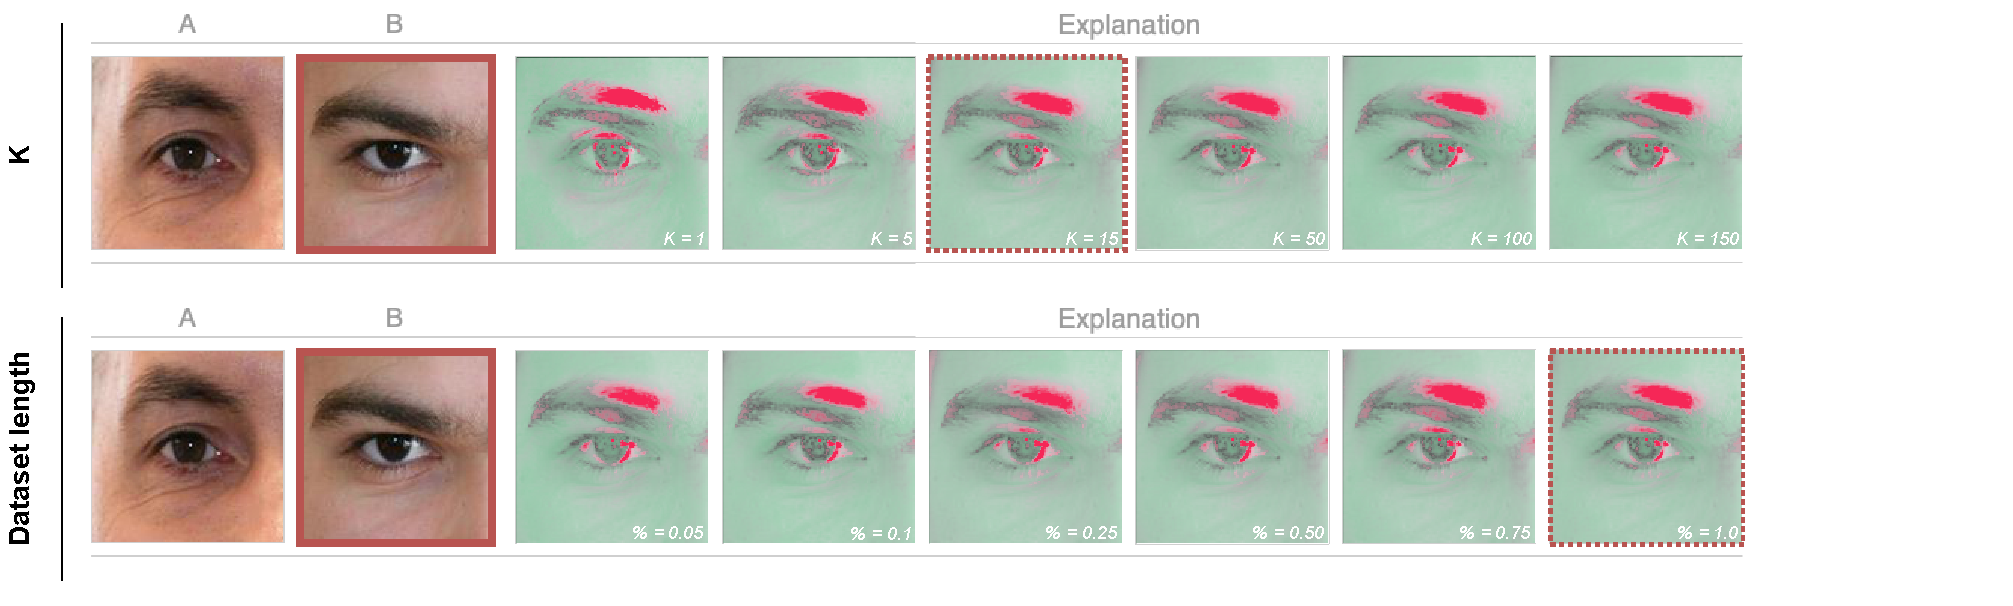
\includegraphics[width=\textwidth]{figures/figure_40.pdf}
  \caption{Typical changes in the results when the two most important parameters of the proposed method are varied. The red square indicates which image is being explained (i.e., $B$), while the red dashed squares provide the default values used in our experiments. In general, increasing $K$ up to $15$ allows for smoother explanations, as does keeping a large dataset. Reducing the latter tends to produce less sensitive results, substantially decreasing the plausibility of the visual explanations.}
  \label{fig:ablation_study}
  \end{center}
\end{figure}

\subsubsection{Number of Neighbours}
\label{subsubsec:chap4_number_of_closest_neighbours}
The value $K$ determines how many synthetic pairs are considered with respect to a query. Overall, we observed that smaller values lead to more sensitive and jagged results. Up to a certain point (e.g., $15$), increasing $K$ typically enables to obtain smoother explanations, due to the larger number of samples taken into account when averaging the closest neighbours. This trend, however, starts returning incremental improvements (notice in Fig. \ref{fig:ablation_study}, where $K>=50$  progressively stops presenting a prominent tone on the eyelid).

\subsubsection{Length of the Synthetic Dataset}
\label{subsubsec:chap4_synthetic_dataset_length}

This is the most sensitive parameter of our solution. Considering that it is important to find "genuine" pairs that closely resemble a query, it is particularly sensitive to assure that all typical periocular data variations are faithfully represented in the synthetic set, assuring that the retrieved elements (i.e., the most similar) will have its major components (iris, eyebrows and eyelids) aligned to the query itself. If this condition is not satisfied, the explanations lose their biological plausibility and effectiveness.
Fig. \ref{fig:ablation_study} illustrates how smaller synthetic sets lead to less evident explanations, especially around the eyelid and the eyebrow. 

\section{Automatic Generation of Image Captions}
\label{sec:chap4_method_b_results}

As the first method, the proposed solution for image captioning attempts to produce explanations that are as easy to understand as possible. With effect, the generated sentences are syntactically correct, following the training distribution, which included many different ways of opening or closing a sentence and conveying the relevant information (i.e., which periocular components sustain an "impostor" decision).

Practically speaking, the first pair has evidently different eyelid shapes and, in the second, the people have obvious differences in the eyebrows (both explanations were included in the generated captions). Next, in the third pair the eyebrow distributions are not different enough so as to justify their inclusion in the explanation (there is a skin spot that could better justify the "impostor" decision). Then, in the fourth pair the explanation returns to a decent accuracy level, by specifying the skins, while in the fifth sample the iris colours are left behind in favour of the skin spots (once again, this is not totally wrong but the spots are perhaps not the most striking visual difference). Finally, the sixth pair is correctly explained by highlighting the skins and eyebrows.

\begin{figure}[H]
  \begin{center}
  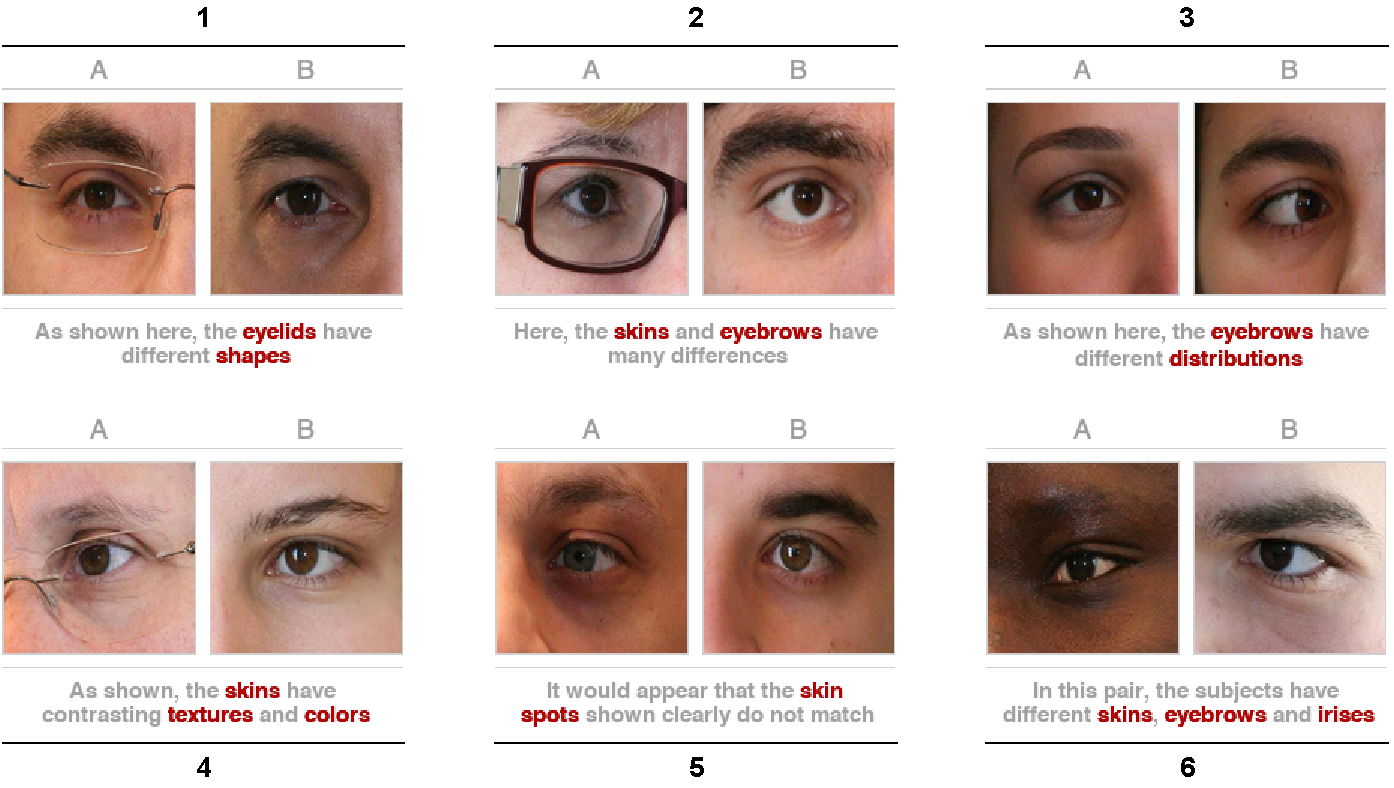
\includegraphics[width=0.90\textwidth]{figures/figure_41.pdf}
  \caption{Samples generated by the proposed solution for automatic captioning. In general, the periocular components (in red) that are included in each explanation are fairly accurate, with some exceptions (e.g., fifth sample).}
  \label{fig:caption_samples}
  \end{center}
\end{figure}

\section{Conclusion}
\label{sec:chap4_conclusion}

The present chapter attempted to validate whether explainability could be achieved in practical scenarios (and in several forms - visual and written, in this case). As seen through the experimental results, both solutions appear to produce satisfactory results (even when the most obvious components are not highlighted, the ones that end up being chosen are not technically wrong). Finally, an interesting possibility would be to combine the two approaches into a single, unified framework that produces more thorough explanations.